\documentclass[a4paper,10pt]{article}
\usepackage[utf8]{inputenc}
\usepackage{graphicx}
\usepackage{float}
\usepackage{amsmath}


\author{Jonathan Teran}
\title{Redes Neuronales - Trabajo Práctico 1}
\date{}

\begin{document}
\maketitle

\section{Introducción}

En este trabajo se propondrán modelos para resolver los problemas propuestos:

\begin{itemize}
	\item Diagnóstico de cáncer de mamas
	\item Eficiencia energética
\end{itemize}

Se explicará como se pre-procesaron los datos de entrada, como interpretar
los datos de salida, y como se obtuvo el modelo final en cada caso.

\section{Diagnóstico de cáncer de mamas}

\subsection{Procesado e interpretación de los datos}

Los datos de entrada de este problema consisten de 10 números reales, y una
salida que puede tomar 2 valores, \textbf{B} (benigno) y \textbf{M} (maligno).

Debido a la magnitud de algunos de los datos de entrada, es necesario
estandarizarlos previamente. Para esto se calculó por cada columna $j$ del
dataset la media y el estimador insesgado del desvío estándar,
y se actualizó cada valor $x_{ij}$ de la siguiente manera

\[ x_{ij} := \frac{x_{ij} - \mu_j}{\sigma_j} \]

, para toda fila $i$ del dataset.

Para la salida, se decidió interpretar un diagnóstico benigno \textbf{B} con
un 1 y uno maligno \textbf{M} con $-1$. De esta forma, podemos usar el signo
de la salida de la red como diagnóstico: para valores $O > 0$ el diagnóstico
sera \textbf{B} y para $O < 0$ será $M$, donde $O$ es el valor que devuelve la
única neurona de salida de esta red.

Tanto nuestros datos de entrada como los de salida pueden tomar valores
positivos y negativos, en un rango que dentro de todo se puede considerar
acotado (entre 1 y $-1$). Es por esto que utilizaremos $g(x) = \tanh(x)$ como
nuestra función sigmoidea de activación.

\subsection{Partición de los datos}

Para verificar que la red sea capaz de generalizar durante la etapa de
búsqueda de un modelo, se decidió particionar el dataset provisto en
sub-datasets de \textbf{entrenamiento} , \textbf{validación} y
\textbf{testeo}, cada uno de tamaño $0.8P$, $0.15P$ y $0.05P$, donde P es la
cantidad de filas en el dataset de entrada.

El dataset de \textbf{entrenamiento} se utilizará para entrenar la red, y el de
\textbf{validación} para comprobar durante y al final del entrenamiento como responde el
modelo ante casos sobre los que no entrenó. Si esta respuesta no es buena, se
cambian los parámetros del modelo para buscar otro mejor. Cuando finalmente la
respuesta es buena, se utilizan ambos datasets para entrenar y el dataset de
\textbf{testeo} se utiliza para calificar a el modelo final, nuevamente viendo
como este responde ante casos desconocidos.

Además, se decidió particionar los datos durante el entrenamiento en
mini-lotes tamaño $B=16$, y calcular la corrección para el modelo como el
promedio de estos. De esta forma podemos acelerar el proceso y aumentar la
cantidad de épocas de entrenamiento sin sacrificar en tiempo de entrenamiento.

\subsection{Modelo final}

Luego de correr el modelo múltiples veces, cambiando parámetros, se concluyó
que una red con 2 capas ocultas, la primera de 20 nodos y la segunda de 8, era
la mejor para resolver este problema. El \textit{learning rate} que se utiliza
es de $0.01$.

Con estos parámetros y luego de 1000 épocas de entrenamiento, se
consiguió un modelo que puede diagnosticar correctamente el \textbf{100\%}
de los casos presentes en el dataset provisto. Si bien esto podría darse por
un \textit{over fit}, recordemos que solamente se utilizaron los datasets
\textbf{entrenamiento} y \textbf{validación} para la etapa de entrenamiento.

\begin{figure}[H]
	\centering
	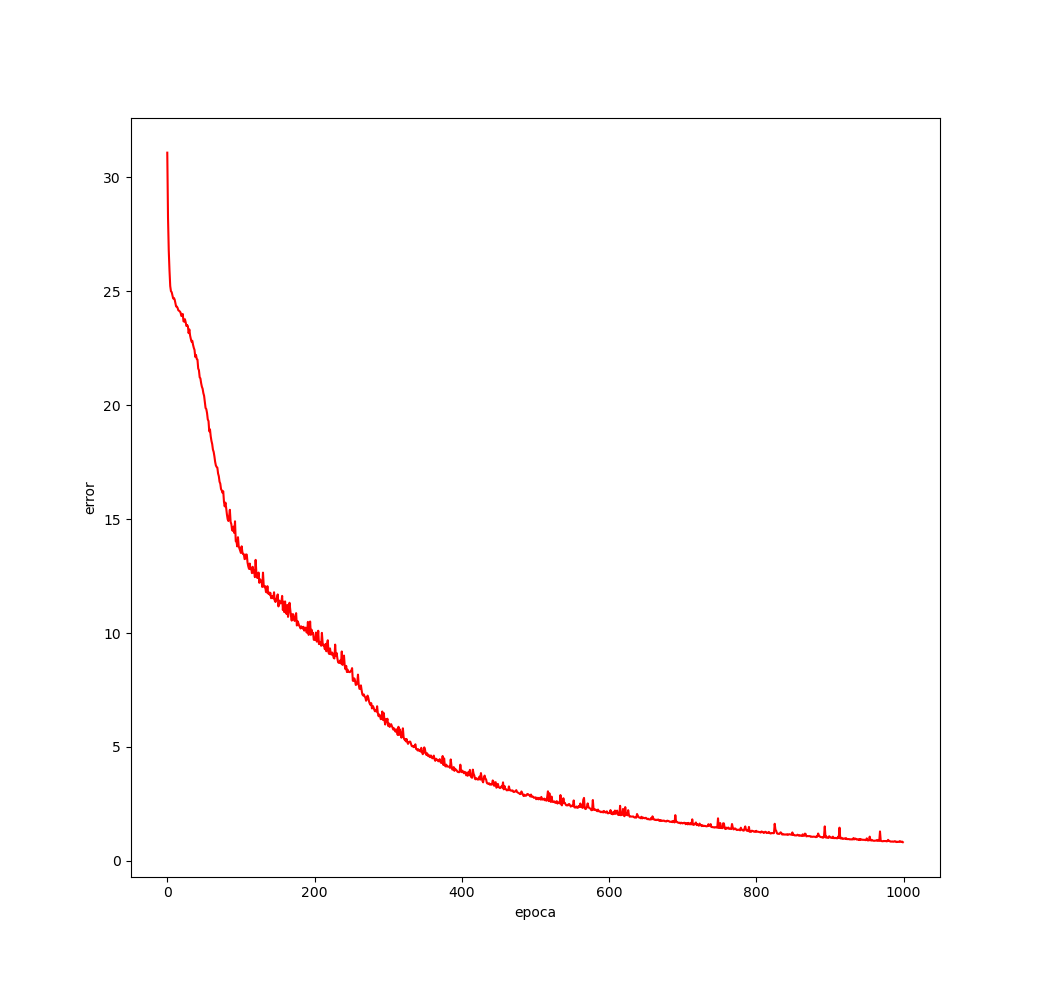
\includegraphics[width=.75\textwidth]{ej1-error_vs_epoca.png}
	\caption{Ej. 1: Error vs Época}
	\label{fig:ej1-e_vs_t}
\end{figure}

En la Figura \ref{fig:ej1-e_vs_t} se puede ver como el error disminuye en cada
época al entrenar un nuevo modelo con estos parámetros.

\section{Eficiencia energética}

\subsection{Procesado e interpretación de los datos}

Al igual que en el problema anterior, el dataset de entrada presenta valores
de magnitudes muy grandes para nuestra red. Los estandarizaremos para obtener
valores mas cómodos.

Sin embargo, en este problema los valores de salida esperados son números, que
nuevamente son muy grandes. Lo que haremos será estandarizarlos y hacer que
nuestra red entrene para producir estos valores en la salida. Luego
desestandarizaremos los mismos, haciendo el proceso inverso:

\[ z_{ij} := z_{ij}\sigma_j + \mu_j\]

, donde $z_{ij}$ es la salida $j$ para la fila $i$.

Otro punto a tener en cuenta es como decidir si la salida de la red es
correcta, o no. Como los valores de salida esperados son reales, resulta muy
difícil que la red produzca estos valores exactos. Por esto, en vez de
comparar la salida de la red con la salida esperada usando la igualdad,
esperaremos que la diferencia entre ambos sea menor que un \textbf{margen de
error}.

Este margen $e$ sera un número real entre 0 y 1. Si el valor de salida es $y$
y el valor esperado es $z$, entonces $y$ se considerará correcto si

\[ \left|\frac{z - y}{z}\right| < e \]

\subsection{Partición de los datos}

Para este problema se utilizaron las mismas particiones que en el caso
anterior, salvo para los mini-lotes de entrenamiento, en los cuales utilizamos
$B=8$.

\subsection{Modelo final}

Durante el proceso de búsqueda de un modelo adecuado para el problema, se
intentó reusar el mismo que el problema anterior. Claramente el desempeño del
mismo fue muy malo para este problema, pero sirvió empezar.

Primero, el error en cada época era muy alto, y decrecía lentamente. Este fue
un indicador de que el \textbf{learning rate} para este problema era muy
chico, y que debíamos aumentarlo. Su valor actual es de $lr=0.5$

Luego, en multiples ocasiones el error permanecía prácticamente constante por
cientos de épocas. Para lidiar con este problema, se agregó un parámetro de
\textbf{momento,} que indicaría que proporción del $\Delta{}W$ del mini-lote
previo se agregaría al $\Delta{}W$ actual. El valor que se utilizó fue $m=0.9$

Con estos nuevos parámetros, el error empezó a disminuir rápidamente en la
primera mitad, pero eventualmente llegaba a un punto en el que crecía y
decrecía de manera alternada. Esto podría darse porque el \textbf{learning
rate} necesario para algunas regiones debe ser más chico que el valor inicial.
Para arreglar este problema, introducimos nuevos parámetros $\alpha$, $\beta$
y $K$ para modificar el learning rate.

Si durante $K$ iteraciones consecutivas se logra disminuir el error, el $lr$
se incrementa en $\alpha$. Si por el contrario, el cambio introducido en la
iteración anterior aumentó el error, $lr$ disminuye en $\beta \times lr$.

\[
	lr = \begin{cases}
		lr + \alpha & \text{si $\Delta E < 0$ durante $K$ iteraciones} \\
		lr - \beta \times lr & \text{si $\Delta E > 0$} \\
		lr & \text{si no} \\
	\end{cases}
\]

Sin embargo después de realizar todas estas modificaciones, el modelo no logró
mejorar su precisión por encima del 75\% de respuestas correctas. Se cambio
la distribución de las capas multiples veces sin éxito.

\begin{figure}
\centering
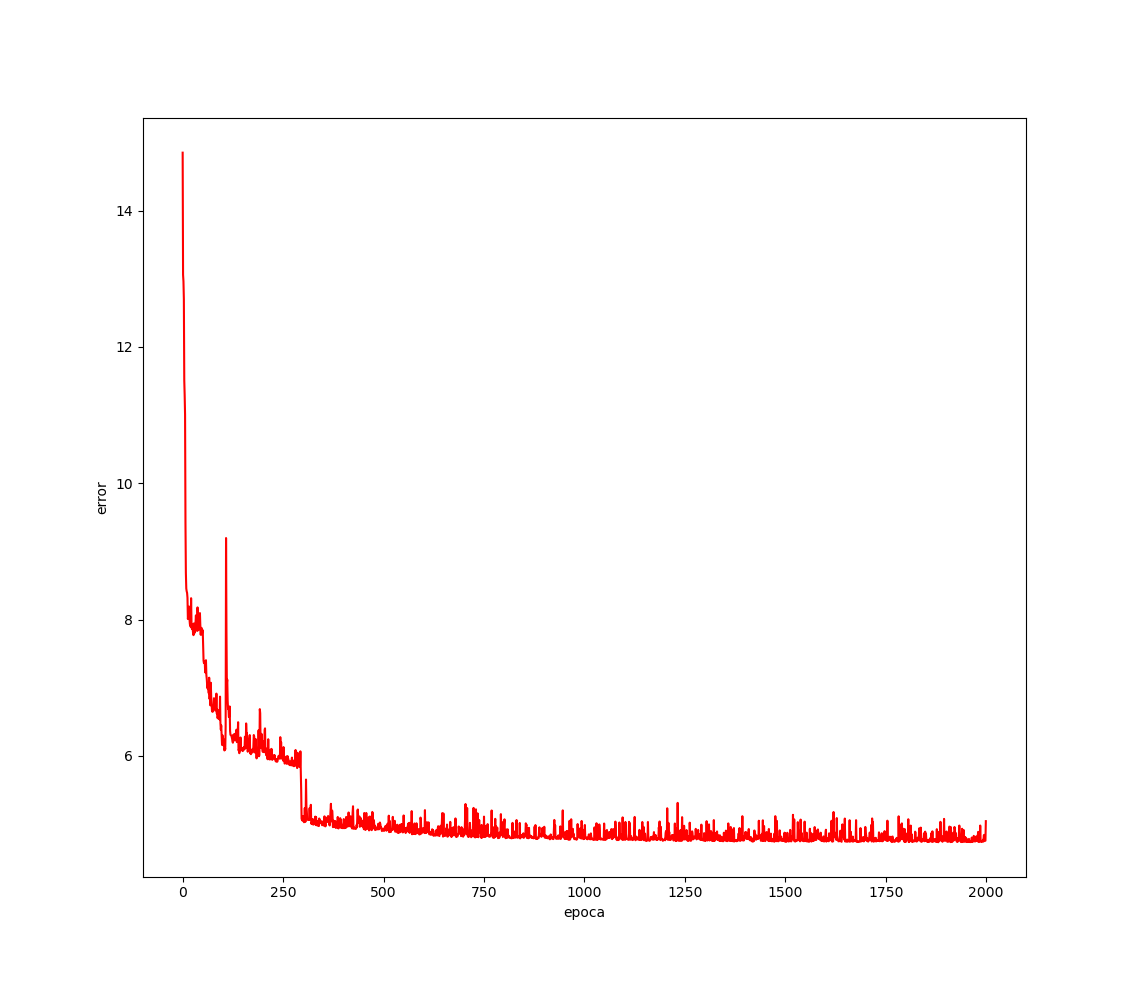
\includegraphics[width=.75\textwidth]{ej2-error_vs_epoca}
\caption{Ej. 2: Error vs Época}
\label{fig:ej2-e_vs_t}
\end{figure}

Podemos observar en la Figura \ref{fig:ej2-e_vs_t} como el error continúa
oscilando a pesar de los cambios introducidos, y como queda estancado después
de la época 250.

Lo más probable es que la configuración que logra minimizar este error, y
aumentar las capacidades de generalizar del modelo exista, solo que no se
logró dar con la misma.

Otro detalle a tener presente es que la precisión puede cambiar fácilmente si
aumentamos nuestro margen de error, que actualmente esta en $e=0.05$. Pero
este valor parece ser razonable mientras que otro mayor como $e=0.1$ o $e=0.2$
deja de serlo.

\section{Conclusiones}

La diferencia en la dificultad de ambos problemas es muy notable. En el
primero fue suficiente con normalizar los datos, encontrar una distribución de
nodos por capa, y aumentar la cantidad de épocas para encontrar un modelo que
obtenga una precisión del 100\%. En cambio, en el segundo problema
introducimos nuevas técnicas para el entrenamiento, nuevos parámetros, y aun
aumentando la cantidad de épocas no se logro aumentar la precisión.

Esto se debe a como se interpretan las respuestas de la red en cada caso. En
el diagnóstico de cáncer de mamas, la red tiene un rango de respuestas
correctas muy amplio, ya que la respuesta se obtiene del signo del nodo de
salida, no del valor del mismo. La red puede producir como respuesta $0.95$,
$0.5$, o $1e-20$ y estos se interpretarán como correctos si el diagnóstico
real fue \textbf{B}. Mientras que en el problema de la eficiencia energética
la red debe producir valores muy precisos para que la respuesta se cuente como
correcta.
\end{document}
